\documentclass{sigchi}

% Use this command to override the default ACM copyright statement
% (e.g. for preprints).  Consult the conference website for the
% camera-ready copyright statement.


%% EXAMPLE BEGIN -- HOW TO OVERRIDE THE DEFAULT COPYRIGHT STRIP -- (July 22, 2013 - Paul Baumann)
% \toappear{Permission to make digital or hard copies of all or part of this work for personal or classroom use is      granted without fee provided that copies are not made or distributed for profit or commercial advantage and that copies bear this notice and the full citation on the first page. Copyrights for components of this work owned by others than ACM must be honored. Abstracting with credit is permitted. To copy otherwise, or republish, to post on servers or to redistribute to lists, requires prior specific permission and/or a fee. Request permissions from permissions@acm.org. \\
% {\emph{CHI'14}}, April 26--May 1, 2014, Toronto, Canada. \\
% Copyright \copyright~2014 ACM ISBN/14/04...\$15.00. \\
% DOI string from ACM form confirmation}
%% EXAMPLE END -- HOW TO OVERRIDE THE DEFAULT COPYRIGHT STRIP -- (July 22, 2013 - Paul Baumann)


% Arabic page numbers for submission.  Remove this line to eliminate
% page numbers for the camera ready copy 

%\pagenumbering{arabic}

% Load basic packages
\usepackage{balance}  % to better equalize the last page
\usepackage{graphics} % for EPS, load graphicx instead 
%\usepackage[T1]{fontenc}
\usepackage{txfonts}
\usepackage{times}    % comment if you want LaTeX's default font
\usepackage[pdftex]{hyperref}
% \usepackage{url}      % llt: nicely formatted URLs
\usepackage{color}
\usepackage{textcomp}
\usepackage{booktabs}
\usepackage{ccicons}
\usepackage{todonotes}
\usepackage{soul}

% llt: Define a global style for URLs, rather that the default one
\makeatletter
\def\url@leostyle{%
  \@ifundefined{selectfont}{\def\UrlFont{\sf}}{\def\UrlFont{\small\bf\ttfamily}}}
\makeatother
\urlstyle{leo}

% To make various LaTeX processors do the right thing with page size.
\def\pprw{8.5in}
\def\pprh{11in}
\special{papersize=\pprw,\pprh}
\setlength{\paperwidth}{\pprw}
\setlength{\paperheight}{\pprh}
\setlength{\pdfpagewidth}{\pprw}
\setlength{\pdfpageheight}{\pprh}

% Make sure hyperref comes last of your loaded packages, to give it a
% fighting chance of not being over-written, since its job is to
% redefine many LaTeX commands.
\definecolor{linkColor}{RGB}{6,125,233}
\hypersetup{%
  pdftitle={SIGCHI Conference Proceedings Format},
  pdfauthor={LaTeX},
  pdfkeywords={SIGCHI, proceedings, archival format},
  bookmarksnumbered,
  pdfstartview={FitH},
  colorlinks,
  citecolor=black,
  filecolor=black,
  linkcolor=black,
  urlcolor=linkColor,
  breaklinks=true,
}

% create a shortcut to typeset table headings
% \newcommand\tabhead[1]{\small\textbf{#1}}

% End of preamble. Here it comes the document.
\begin{document}

\title{Supporting Collaborative Information Analysis: A Classroom Study}

\numberofauthors{3}
\author{%
  \alignauthor{1st Author Name\\
    \affaddr{Affiliation}\\
    \affaddr{City, Country}\\
    \email{e-mail address}}\\
  \alignauthor{2nd Author Name\\
    \affaddr{Affiliation}\\
    \affaddr{City, Country}\\
    \email{e-mail address}}\\
  \alignauthor{3rd Author Name\\
    \affaddr{Affiliation}\\
    \affaddr{City, Country}\\
    \email{e-mail address}}\\
}

\maketitle

\begin{abstract}
% abstract

Collaborative information analysis involves strategic analysis and representation of complex information space through synchronous and asynchronous team interactions over extended time periods. Chances are rare to observe how technology affects analysts on collaborating on complex information analysis tasks because such scenarios are difficult to model in lab studies, and are often limited to access in real world. Classroom study provides a testbed in which students are trained to become professional analysts and course projects are designed to simulate real world tasks. We deployed our tool, a collaborative visual analytic tool informed by earlier work, in class and observed the usage of the tool by teams in their project. Particularly, this paper reports how analysts-in-training used the tool in evidence collection, evidence schematization, hypothesis generation, and overall coordination, four critical parts in the task of collaborative information analysis. The paper ends with discussion over several theoretical and design implications.
%
%Collaborative information analysis typically involves representation and analysis of complex information space through synchronous and asynchronous team interactions over extended time periods. It is important to examine, understand, and provide effective tools and environments for these long-term, real world CSCW interactions. We have developed a tool, CAnalytics, to support collaborative information analysis through coordinated multiple views, to raise user awareness through real time sharing and other mechanisms, and to facilitate communication with an enhanced messaging tool. We deployed CAnalytics in an intelligence analysis course, in which 76 analysts-in-training used our tool for a one-week-long project. We report users' experience in this paper. Participants found the tool facilitated their teamwork and increased their engagement, but they also experienced breakdowns. The paper ended with discussion over design implications we derived from the field study.
\end{abstract}

\keywords{Collaborative information analysis; visualization; classroom study;}

\category{H.5.3.}{Information Interfaces and Presentation
  (e.g. HCI)}{Computer-supported cooperative work} 

% introduction
\section{Introduction}
\hl{not modified yet}

Collaborative information analysis is a form of sensemaking wherein a team analyzes a complex information space of facts and relationships to identify and evaluate causal hypotheses. A common example of collaborative information analysis is crime investigation; a variety of putative facts are assembled, including financial records, witness observations and interviews, and social connections of various sorts among persons of interest, from which investigators collaboratively  assess means, motives, and opportunities, articulate and investigate further hypotheses and deductions, and develop one or more theories of the crime. Other examples include intelligence analysis, business intelligence, scientific research, and social constructivist learning. Collaborative information analysis tools are designed to support such tasks.

However, Evaluation of collaborative tools is challenging for several reasons. For example, participants could address information in a qualitatively different manner. Participant's education, past experience, role requirement, cultural values, and organizational norms strongly influence the way they perceive information, what they perceive, and how they respond to this information \cite{heuer1999}. Therefore professional information analysts could have different strategies accomplishing a task and thus different perspectives toward the tool from casual users. Professional analysts have knowledge of practice of community such as structured analytic skills that is unavailable for untrained people. The problem is, however, professional information analysts such as intelligence analysts are often limited to access due to security issues. It is difficult to have them in a design loop and conduct a long term design research. 

Another challenge is to model the complex collaborative information analysis task as it is in reality. In a crime investigation situation, for example, teams interact with each other for weeks or months. During the period, analysts having multiple threads going on simultaneously. Issues that were raised an hour ago, or a week ago, may nonetheless be critical again. Collaborators need to keep track of how their teamwork is organized and managed, including team strategies and practices, and interdependent member responsibilities and roles. Analysts may be located in different places, and may have to work asynchronously together. All such complexity, while extremely common in real world, can hardly be modeled in lab study.



% Analysts seek to identify entities of interest from mass information and to determine relationships beyond those literally specified in the original data. A common example is crime investigation; a variety of putative facts are assembled, including financial records, witness observations and interviews, and social connections of various sorts among persons of interest, from which investigators collaboratively  assess means, motives, and opportunities, articulate and investigate further hypotheses and deductions, and develop one or more theories of the crime. Many critical problem domains beyond crime investigation involve or are examples of collaborative information analysis, including intelligence analysis, scientific research, and social constructivist learning.

% % BVH: mention supporting collaborative IA, raising awareness, and facilitating communication
% % DONG: modified the following paragraph to reflect the three elements.
% Collaboration is vital to information analysis. Prior studies \cite{Chin2009, Kang2011} have emphasized that the work of information analysis at non-trivial scales is fundamentally collaborative. However, the state-of-the-art analytic tools that are currently wide used, such as IBM Analyst's Notebook, and PARC ACH, are designed for individual use only. For successful collaboration, awareness of teammate's activities and effective communication is critical. Without effective support, analysts have to coordinate their work by manually sharing their work. The fact that the single person operating the software is observed to be a bottleneck to the team process \cite{Rosettex2004}. Tools to support and mediate such collaboration is critical; in particular, we need tools to support information analysis, to raise user awareness, and to facilitate communication.

% Besides, evaluation of collaborative tools is challenging, due to difficulty in data collection, number and complexity of variables, and the challenge to evaluate in real context \cite{Neale2004}. Real world information analysis often extends over long time periods involving synchronous and asynchronous team interactions, which can hardly be modeled in lab experiments. This requires situating research in more complex work activity contexts. On the other hand, however, professional information analysts in real world are often within limited access due to security and privacy issues. Attempts to observe their work and involve them in long-run iterative design is almost impossible. 

% To address these concerns and to support collaborative information analysis with complex tasks, we have developed a collaborative information analysis tool and deployed it in a naturalist environment. The design of the tool is informed by prior experiments of teams collaboratively analyzing crimes cases using paper prototype \cite{}, by field studies conducted by Chin \cite{Chin2009} and Kang and Stasko \cite{Kang2011}, and by existing systems \cite{Jigsaw2008, Bier2010}. The tool supports identifying analytic entities through document annotation and connecting and presenting information through multiple coordinated visualizations. We also built a set of features to increase user awareness, such as real time update of user created objects, an integrated notification system, and peripheral user working area indicators, and a dedicated user activity history.

In this paper, we reported a classroom study to evaluate a tool we developed for collaborative information analysis. We deployed our tool in an intelligence analysis course project in a US university. As an alternative to professional analysts, our participants are all analysts-in-training, who are learning state-of-the-art analytic skills and are soon to become professional intelligence analysts. They are familiar with the practice of the intelligence community and are instructed to follow that practice in their course project. The project task simulates real world intelligence tasks and requires teams to devote serious efforts to develop and valid hypotheses based on given materials. Students switch regularly back and forth between other course assignments and this project, and must accomplish the project under limited time and resources, similar to the real world situations of intelligence analysts. Students are graded in the course on their ability to understand and enact professional practices of information analysis. This strong normative emphasis on problem solving practices is a great evaluation context for new interactive tools: Tools are only valuable to the students insofar as they actually support better practices and better outcomes.

Particularly, we focus on the tool effect on three aspects: support for information analysis, support for activity awareness, and support for communication. Information analysis includes information gathering and synthesis, as well as hypothesis development and validation. Prior studies \cite{Chin2009,Kang2011,Borge2012} identified several requirements for effective information analysis, such as visual representation of data relationships, use of multiple variables to for data reduction, insight provenance for sanity checks, etc. Activity awareness \cite{Carroll2003} is a key enabler for effective collaboration. Collaborators need to keep track of what their partners have done, what they are doing, where they are working on, and their relevant experience, distinctive resources and unique knowledge, prior contributions and perspectives, as well as values, expectations, and goals. Finally, communication helps team coordinate and exchange opinions. Effective communication makes a team feel on the same page whereas ineffective communication wastes a lot of time in clarifying misunderstandings. We observe students' performance on these aspects and discuss the role of our tool in supporting or hindering them. 

Our work will be beneficial to design researchers and information analysis practitioners. Prior works have examined team behaviors in collaborative information analysis using state-of-the-art tools (current practice) \cite{Kang2011,Chin2009} or with low-fidelity tools (e.g. paper and pen) \cite{Borge2012}, or in a simplified laboratory task \cite{Goyal2016}. Our work is the first to observe team behaviors mediated by advanced technology in a naturalist environment, thus providing a more realistic picture of how tools are appropriated in team collaboration. 

A broader impact we anticipate is to contribute to technology-enhanced education of intelligence analysis. Methods in the intelligence community remain largely unchanged over the last few decades, and analysts are often trained with traditional methods. Our work is a starting point to bring advanced technology to intelligence training. It is important not only because it is likely to help students to learn and practice analytic skills in a more effective way, but more significantly, it opens up new possibilities for these future intelligence analysts to approach collaborative information analysis and encourage them to in turn push forward the development of technology in the area. 

% On the one hand, students employed our tool as an alternative to mediate their project activities; on the other hand, it served as a large-scale testbed for our tool. We report students' response to the tool and discuss design implications we find from the result.

% % TODO: cite Heuer to argue the importance of participants in information analysis
% ``What people perceive, how readily they perceive it, and how they process this information after receiving it are all strongly influenced by past experience, education, cultural values, role requirements, and organizational norms, as well as by the specifics of the information received.'' \cite{Heuer2006}


% related work
\section{Related Work}
\hl{not modified yet}

% need for collaborative information analysis
The i2's Analyst's Notebook and and PARC ACH \footnote{Analyst's Notebook: http://www-03.ibm.com/software/products/en/analysts-notebook, ACH: http://www2.parc.com/istl/projects/ach/ach.html}are widely used tools for information analysis, and emphasize support for visualizing events in temporal themes and for competitive analysis of alternative hypotheses, respectively. Recent research has focused on visualizing entity and relationships both more directly, from the user's standpoint, and through multiple view techniques. Entity-based systems such as the Entity Workspace \cite{Bier2010} and Jigsaw \cite{Jigsaw2008} extracts data objects including people, location, and times, and represent them in organized graphical structures. All these systems attempt to reduce the cost of manipulating text into connected data objects. 

However, these tools lack serious collaboration support. Analysts must coordinate work by manually sharing notebooks or graphs. This has the consequence that the tools are employed only at specific points in an analysis, often only in the early stages during which analysts are working on their own. Indeed, the use of these tools directly diminishes a team's awareness, requiring repeated manual resynchronizing to identify redundant or missing pieces of information, analysis of information, and analytic hypotheses. The instructor and students in our study were also aware of the shortcomings of available tools with respect to support of collaboration.

Carroll and his colleagues \cite{Borge2012, Carroll2013} conducted a lab experiment and observed how teams collaboratively analyzed information using paper prototype. By analyzing team process and artifacts teams developed, they derived design suggestions for mediating tools.  Goyal et al. \cite{Goyal2013, Goyal2014, Goyal2016}  reported several lab experiments investigating the effect of individual tool features on collaborative information analysis. Their work provides evidence of tool effect on collaboration. Other studies have been conducted to examine the technology to support group awareness. 
% TODO include citations 
These technologies include visualizations of working areas of collaborators \cite{Gutwin1996}, highlighting of changes \cite{Hajizadeh2013}, notification systems \cite{Carroll2003}, and historical activity list \cite{Ganoe2003}. These studies were all conducted in lab experiments, which focus on relatively simple tasks and short periods of time. As task complexity increases and time expands, however, team behavior could be qualitatively different. % TODO citation

% BVH Changed this from using passive voice
Researchers have conducted several field studies aimed to understand design requirements of collaborative information analysis in more realistic setting. Chin et al. \cite{Chin2009} conducted an observation study of professional intelligence analysts, and examined the strategies and tools they applied. Their study is important as it sheds light on how real professionals work. In practice, access to professional analysts over an extended period of time is often restricted due to safety and privacy issues. As an alternative, Kang and Stasko \cite{Kang2011} studied how student analysts---who were soon to become professionals---completed in-class intelligence projects using state-of-the-art tools. This approach proves to be a practical way to understand and involve users in the problem space. Our study followed this approach, and took one step further; we deployed our tool in an intelligence analysis course and took advantage of the course as a large-scale testbed to investigate the tool we have developed. 


% system



%i2's Analyst's Notebook
%
%Stasko, J., Görg, C., & Spence, R. (2008). Jigsaw: supporting investigative analysis through interactive visualization. Information Visualization, 7(2), 118–132. http://doi.org/10.1057/palgrave.ivs.9500180
%
%Bier, E. a., Card, S. K., & Bodnar, J. W. (2008). Entity-based collaboration tools for intelligence analysis. In 2008 IEEE Symposium on Visual Analytics Science and Technology (pp. 99–106). Ieee. http://doi.org/10.1109/VAST.2008.4677362
%
%
%% empirical study, including lab experiment and longitudinal field study, and evaluation method
%
%professionals are difficult to access for longitudinal observation
%
%% awareness issue
%
%% evaluation
%
%Carroll, J. M., Borge, M., & Shih, S. (2013). Cognitive artifacts as a window on design. Journal of Visual Languages & Computing, 24(4), 248–261. Retrieved from http://www.sciencedirect.com/science/article/pii/S1045926X13000207
%
%Borge, M., Ganoe, C. H., Shih, S.-I., & Carroll, J. M. (2012). Patterns of team processes and breakdowns in information analysis tasks. In Proceedings of the ACM 2012 conference on Computer Supported Cooperative Work - CSCW ’12 (pp. 1105–1114). New York, New York, USA: ACM Press. http://doi.org/10.1145/2145204.2145369
%
%Goyal, N., Leshed, G., Cosley, D., & Fussell, S. R. (2014). Effects of Implicit Sharing in Collaborative Analysis. In Proceedings of the Proceedings of the SIGCHI Conference on Human Factors in Computing Systems (pp. 129–138). Retrieved from http://www.cs.cornell.edu/~ngoyal/1470_Chi2014.pdf
%Goyal, N., & Fussell, S. R. (2016). Effects of Sensemaking Translucence on Distributed Collaborative Analysis. In CSCW ’16 Proceedings of the 18th ACM Conference on Computer Supported Cooperative Work & Social Computing.
%Goyal, N., Leshed, G., & Fussell, S. (2013). Effects of visualization and note-taking on sensemaking and analysis. In CHI ’13 Proceedings of the SIGCHI Conference on Human Factors in Computing Systems (pp. 2721–2724). Retrieved from http://dl.acm.org/citation.cfm?id=2481376
%
%Chin Jr, G., Kuchar, O. A., & Wolf, K. E. (2009). Exploring the analytical processes of intelligence analysts. In Proceedings of the SIGCHI Conference on Human Factors in Computing Systems (pp. 11–20). Retrieved from http://dl.acm.org/citation.cfm?id=1518704
%
%Kang, Y., & Stasko, J. (2011). Characterizing the intelligence analysis process: Informing visual analytics design through a longitudinal field study. In 2011 IEEE Conference on Visual Analytics Science and Technology (VAST) (pp. 21–30). Ieee. http://doi.org/10.1109/VAST.2011.6102438



\section{Classroom Study Settings}

The context for this study was an undergraduate course with an enrollment of 98 students in two class sections, in an intelligence training program in a US university. The program was designed to train students to become professional intelligence analysts. All the students were majoring in the program. 73 students consented to our study protocol and agreed that their data be collected and analyzed. They were randomly assigned to small teams of three (two teams were made of three members) making up 25 teams in total. Most (75\%) of them are in the third academic year (3.05 years in average), indicating that participants in our study have relatively advanced experience and knowledge in intelligence analysis. Participants' age ranges from 19 to 28 (20.3 in average). 77\% of the participants are male. The other 25 students opted out of the study (did not submit the consent form), thus their data was excluded from the analysis.

A key requirement of the course is to emphasize hands-on practice on team-based intelligence analysis. During the first nine weeks, students were taught several structured analytic techniques, such as ACH and network analysis, and instructed to utilize PARC ACH and IBM Analyst's Notebook to solve exercise projects.

Students used CAnalytics for a one-week-long project. The project task is to find the robber(s) in seven hypothetical bank robberies fabricated by the course instructor. Students were provided with documents describing information from witnesses, video records, and news media. Students needed to not only identify the key entities in the documents but also infer possible links between entities and across robberies. The result of the task is open-ended, which means that there is no single answer to the task. Participants must make full use of the provided materials and make their best hypotheses based on evidence. This situation is very similar to real world settings and adds to the complexity of the task. The study is administered in the ninth week of the course. Before then students had learned all analytic theories and strategies (e.g. ACH, IEW) taught in that course and had hands-on experience on some state-of-the-art tools, such as IBM Analyst's Notebook and PARC ACH. The instructor told the students that a minimum of 6 hours was expected to complete the project, including in-class and outside-class work. By the end students were required to submit a group report, describing their findings and supporting evidence.

Students were given a tutorial on CAnalytics a week before the project began. One of the authors first walked students through features of CAnalytics and then let students accomplish a small case analysis themselves to ensure everyone was comfortable with the tool. When the project started, one author was always available to help with any technical issues. Although students were encouraged to make full use of CAnalytics, to ensure a naturalist environment they were always free to apply any other tools that they believed to be useful to their work. . 

In total, 73 students were enrolled in the study from two course sessions. Students were assigned randomly by the instructor into small groups of three members (two groups were made of two students), therefore 25 groups. The rest of the students in the course (25 students) opted out of the study. They employed analogous methods (Analysts' Notebook, ACH, etc.) for the project, but their data is excluded in the analysis.



Our collected data includes three aspects: 1. a post-study questionnaire, 2. system log, and 3. team report. In the questionnaire, we includes several 7-index questions measuring individual's self-reported awareness \cite{Convertino2011}, perceived performance \cite{Goyal2014}, and usability (using SUS \cite{}). The questionnaire also includes several open-ended questions asking how the tool helped or impeded their work. 

The system log is carefully designed so that we capture high-level user activities instead of mouse events and keyboard strokes. For example, we log when the user creates, updates, reads, and deletes an entity. We also log which tool the user is working with. Table~\ref{table:log_schema} shows the schema we use for the log system.  

Although there is no single answer to the task problem, there exist several pieces of key evidence that suggest links across different robbery cases. Together with the course instructor (also the creator of the project task), we designed a rubric for grading. For example, whether they captured that Case 3 and Case 5 is much likely to be committed by the same group of robbers; whether they captured that a ``copycat'' in Case 6? The team get one point when they discussed that hypothesis, and get one point when they provide reasonable evidence.

As suggested by prior works \cite{Neale2004,Goyal2014}, we employed a battery of measures in the study. We administrated two mid-surveys, each at the end of the class, immediately after they finished working in class. The mid surveys measure their self-reported awareness, including their awareness of what teammates have done in the past, what they are doing, and what they are going to do, as well as their awareness of the overall group goals and plans. During class, 15 groups were randomly selected to be observed by research assistants. Assistants were required to only silently observe and take notes and not to interfere participants. At the end of the project, we administrated a post-survey, repeatedly measuring their self-reported awareness. The post survey also includes several open-ended questions about their use experience and difficulty in the process.



% demographic information


\section{CAnalytics}
\begin{figure*}
	\centering
	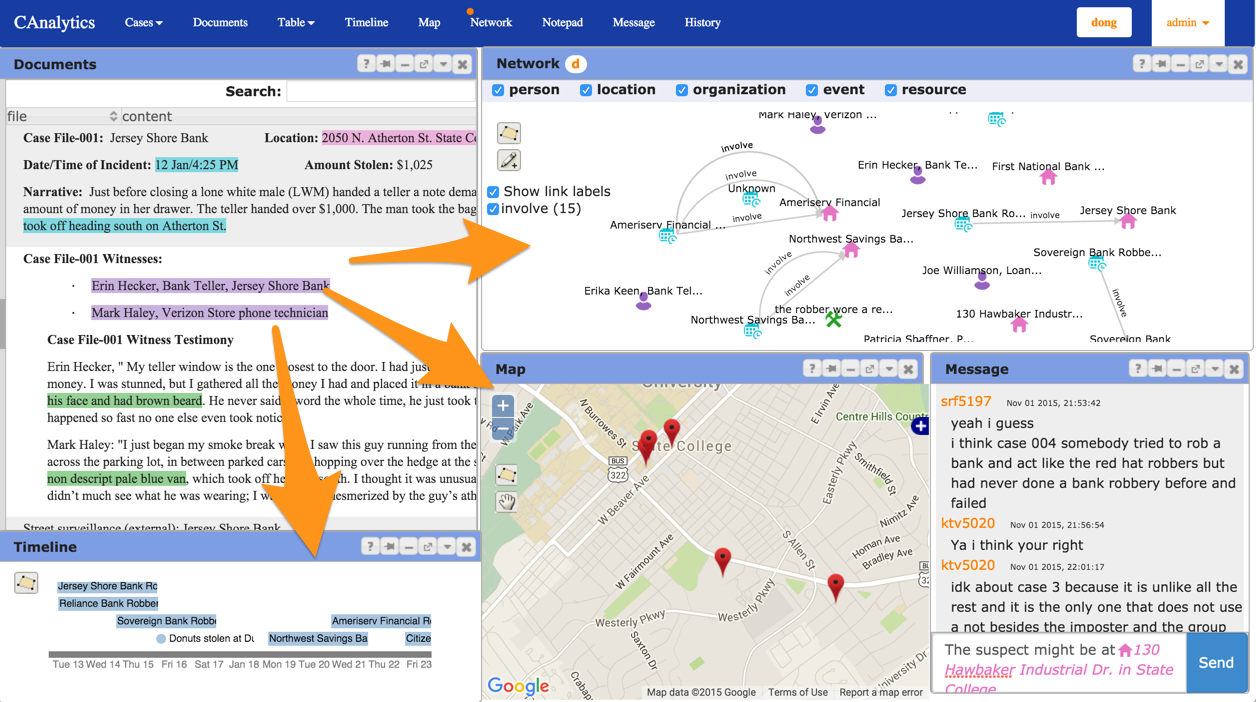
\includegraphics[height=3in]{img/ca_annotation}
	\caption{CAnalytics user interface}
	\label{fig:canalytics}
\end{figure*}

We developed a collaborative information analysis tool, CAnalytics, to support distributed teams of analysts in identifying, visualizing, integrating and assessing facts from multiple sources. The design is informed by existing entity-based information systems \cite{Bier2010} and real-time collaborative systems \cite{Goyal2014}, as well as by findings of prior paper prototype studies of teams performing information analysis tasks \cite{Carroll2013}, Chin et al's \cite{Chin2009} study of intelligence analysts, and Kang and Stasko's \cite{Kang2011} field study of analysts-in-training. The following are explicit design choices we made to enhance collaborative evidence collection, collaborative evidence schematization, and overall coordination and communication respectively. 


\subsection{Semantic annotation for evidence collection}
CAnalytics supports evidence collection through annotation. In the document view users can highlight and annotate information about people, location, events, etc., as well as relationships between them. Unlike in other entity-based systems e.g. \cite{Bier2010}, we use manual annotation for objects of interest. This allows for greater user control in information gathering. Users can decide their own information granularity and information interest that best suits their ad-hoc analytic needs. 

We call it ``semantic'' annotation because the annotation is not only a highlight mark on document text (as usually is), but users can add attributes to annotations, e.g. add time attribute in event, coordinate in location. Thus each annotation is a data object that embeds information of evidence entity. Users can also make reference to other objects in the attribute; for example, users can add people objects involved in an event. A few utilities are available to facilitate data input, e.g. geocoding address, auto-completion of existing data objects. Annotation also records the source where a data object was created---users can always re-access the data objects in its original context of the problem document, a critical requirement emphasized by \cite{Chin2009}.

Our tool supports real-time collaborative editing, similar to the Google Tools. Users can open several concurrent editors to collaboratively edit multiple annotations and events. User created data objects are immediately shared within a team. As far as we know, this tool is the first to support multi-concurrent editing, which we think can improve fine grain coordination and awareness in complex collaborative work. The tool also includes a notepad, in which users can collaboratively compile a document, similar to Google Doc. 

In sum, users accomplish three things when creating an annotation: 1. highlight critical information in the document; 2. model data objects in preparation for later visualization and analysis; 3. connecting data object with source of document for evidence provenance. Annotations are synchronized in real time for collaborative evidence collection. 
	
\subsection{Multiple coordinated views for evidence schematization}

CAnalytics supports information analysis by automatically organizing user created objects in multiple coordinated views, including table, timeline, map, and node-link graph---tools that are most frequently used in information analysis tasks \cite{Carroll2013}. Each visualization provides a way to schematize data: timeline organizes data by time, map by location, node-link graph by relationships, and table by attributes. Figure \ref{fig:canalytics} shows an example of the multiple visualizations in our tool: when an annotation is created in the document module, with information about time, location, participants, and their relationships, a new event is created in the timeline module, a new location is created in the map module, and new people are created in the node-link graph module with a typed edges representing relationships among the people (or new edges are added to existing nodes). 

Different views are coordinated; that is, when users do a filter on a piece of information in one views, related information in other views will be highlighted. Filtering on different views/schematization provides different analytic strategies; e.g. timeline offers filtering by time, map offers filtering by location, and node-link graph offers filtering by related data objects.

Based on default view of evidence, users can continue to schematize it. For example, users can drag the nodes in the node-link graph to make clusters. Users can also create a relationship in the graph by drawing a link between two nodes and input relationship attributes. 

\subsection{Awareness features for coordination}
	
CAnalytics has a number of awareness features, including real time data sharing, a notification system,  a design we named ``tool coordinator'', a message tool, and a history tool. As mentioned before, annotations and data objects created by collaborators are immediately shared. Annotations will be highlighted in the exact position on teammate's document view, indicating which part of the document teammates are working on. Data objects will be visualized in multiple views together with existing data, keeping latest gathered information available to the team. A notification system sends individual's actions to the team, in the form of a text box in the top right corner of the workspace, keeping the team up to date with collaborator's actions. To reduce notification noise, instead of broadcasting whatever actions, we define a set of rules to determine which actions will be notified. For example, the action that creates an entity will be notified, but that re-layouts a view will not. Tool coordinator refers to a small indicator on the tool menu bar, suggesting who is working on the tool. 

The message tool enables real time team communication. Chat history is also persistent for traceability. We design a ``mention'' feature---users can refer to created entities and relationships in the workspace when they are composing a message. We believe this will improve communication efficiency because analysts are often observed to mention critical information entities in face-to-face discussion. \cite{Carroll2013}. When the message receiver hovers over the object, attributes of the object shows up, ensuring that the team is talking about the same thing (as \cite{Carroll2013} observed, one frequent collaboration breakdown is misunderstanding of the object in discussion). 

The system maintains a persistent log of time-stamped individual activities. A history tool presents who did what to which object at when. Together with the notification system, users who work synchronously can be informed of others' activity continuingly, and be aware of the bigger picture of team's activity; users who work asynchronously will be able to use the history to reconstruct their work status and become aware of changes beyond the point of their last interaction. 
		
Different from awareness features developed in existing systems which are simply read-only text, the awareness information in our system is closely integrated with the analytic environment. For example, data objects that are changed and presented in the history view are clickable links. Users can hover over to read detailed attributes and click to do a filter on the object.  
		

The system also includes a simple notepad implementation to support collaborative hypothesis generation. We integrate Etherpad \footnote{Etherpad url}, an open sourced collaborator editor much like Google Doc, for teams to compose their hypotheses. Users can insert tables (e.g. an ACH matrix) and images (views of evidence schematization). However, by the time of this study, we have not developed any advanced features specific for the task of information analysis, and usage of the editor for hypothesis generation is not the emphasis of this paper. 



% results
\section{Result}


\subsection{Usage Overview}

\begin{figure*}
	\centering
	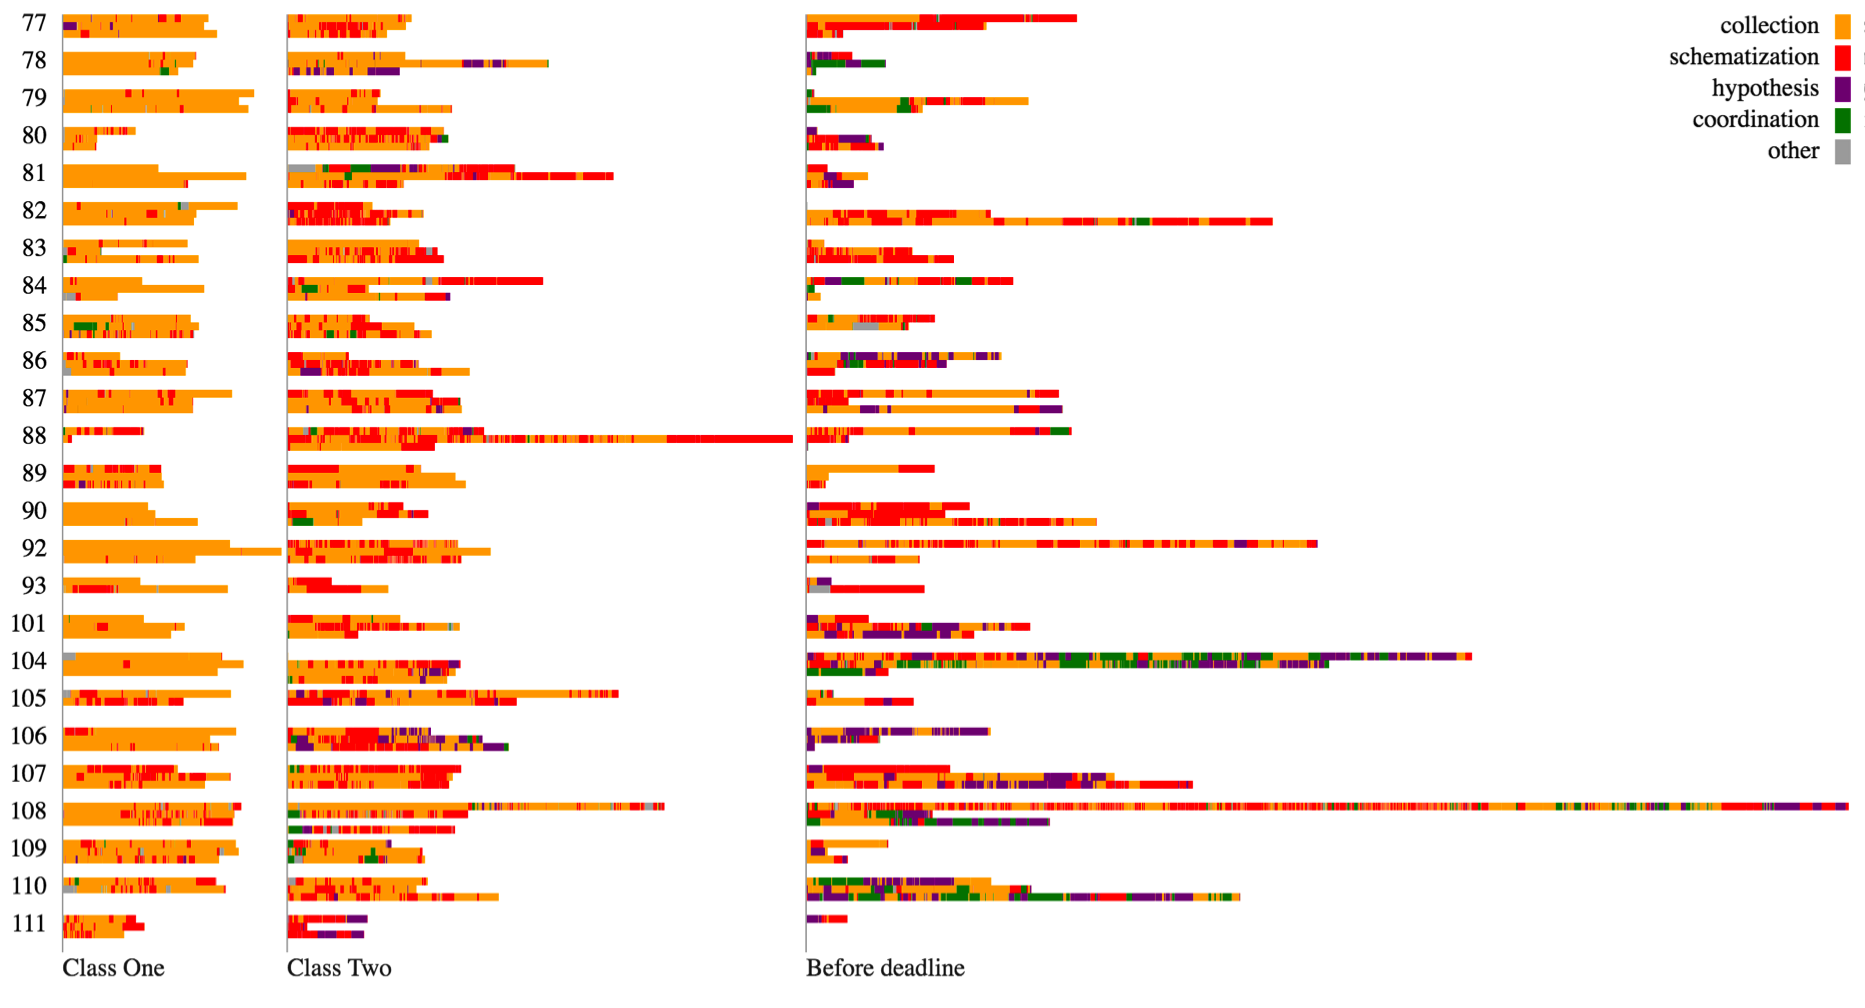
\includegraphics[height=2.5in]{img/phase_sequence}
	\caption{Teams' activity patterns of evidence collection, evidence schematization, hypothesis generation, and overall coordination.}
\end{figure*}



From the system log we made an approximation of the time teams spent on each phase (Figure~\ref{fig:phase_time}). Note that there could be multiple error sources. For example, we actually only capture discrete log events on a tool, and we approximate the duration time assuming that the user keeps on working on that tool until the next log event occurs on another tool (but we discard the time if the interval between two log events is bigger than a threshold). Also we assume that people working with annotation are in evidence collection, and people working with visualizations are in evidence schematization, but in fact no clear boundary exist between the phases. For instance, participants might be schematizing and analyzing evidence as well when they are reading documents and making annotations. 

Yet still, there are several things we can learn from such approximation. For instance, nearly all teams spent most time on tools for evidence collection, less on tools for evidence schematization, and least on tools for hypothesis generation. This seems in contradict with theory; people should spend more time on high level sensemaking activities and focus on the problem itself rather than the underlying data. While evidence collection itself is time-consuming as it requires large amounts of manual input, more advanced input facilities is needed to reduce the time in this phase. 

We use time spent on the history tool and message tool as proxy of overall coordination, although it is only a small portion in real team coordination, because teams can talk directly face-to-face in our study. 

From the system log, we can clearly see that user activities are most intense in three time periods: during class one, during class two, and before project deadline. In class time, students are obviously working together; but when outside class, teams have different choices. 


\begin{figure}
	\centering
	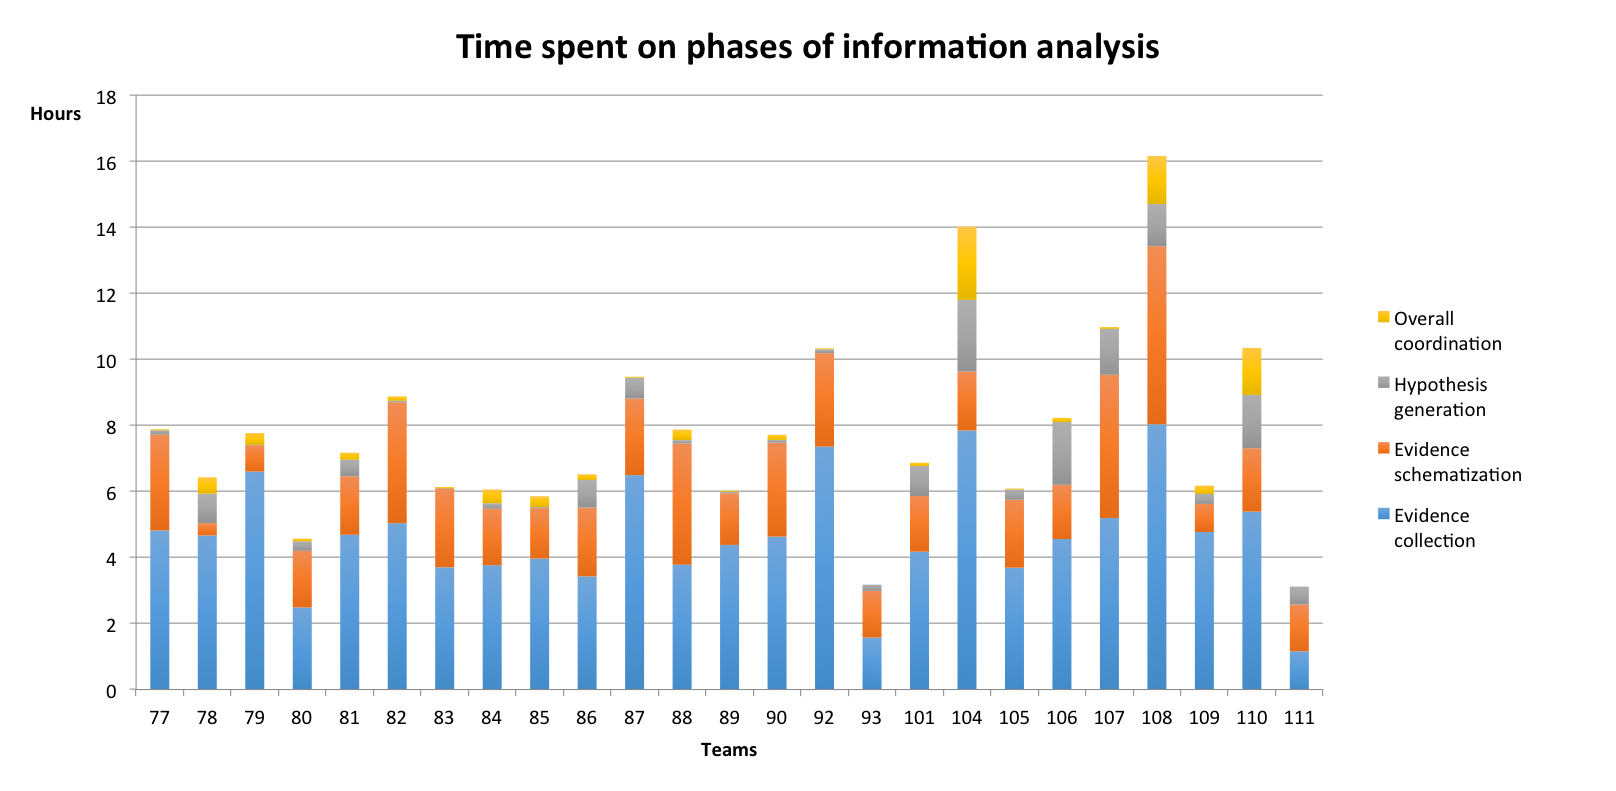
\includegraphics[height=1.5in]{img/phase_time}
	\caption{Time spent on each phase of information analysis.}
\end{figure}

We then look in more detail into the sequence of user activities, in an attempt to find if there exists any behavior patterns between teams, as shown in Figure~\ref{fig:phase_sequence}. Since there are obviously three active usage periods, we align activities into three phases: in the first class, in the second class, and before project deadline. Note that this graph only shows the order of activities performed by participants and spare time between activities (if any) is removed to reduce graph sparsity. We find that teams tend to have a behavior swift between phases. In the first phase, teams spent most time in evidence collection. In Phase Two, teams started to engage in evidence schematization. And teams apparently worked more in hypothesis generation activities. For teams working remotely, they also utilized coordination tools. 

Unlike the sensemaking model \cite{?}, which implies a linear process in information analysis (analysts first specify problems and requirements, then collect information, followed by schematization and analysis, and finally produced a report), we find that teams have a more flexible workflow. They do not wait until all information is collected to do analysis, nor do they hold generating hypotheses until analysis is done. Especially starting from Phase Two (and some teams started even earlier e.g. Team 107) when teams felt they had collected ``good enough'' evidence, they started to use the visualization tools and hypothesis tools. And they switch back and forth from one activity to the other frequently. Especially in later stage, teams seemed to work on the three activities in parallel.  

\hl{TODO: describe the pattern in more details}

In students' reflection, they believe that the integrated analytic environment that CAnalytics provides makes their work more effective and efficient. 

\begin{quote}
	When we didn’t have CAnalytics, we had a lot of different word documents that we had to share with each other in google documents. (P155)
\end{quote}

\begin{quote}
	our team is doing better because CAnalytics as a whole lets us see, analyze, and make conclusions all within one location. (P123)
\end{quote}







\begin{quote}
	\textit{`CAnalytics seemed like the beta-version of an analyst's notebook that multiple people could work on at once...It was like having an analyst's version of a Google Doc.'} (P21)
\end{quote}






\begin{quote}
\textit{`It was much easier to coordinate as a team with CAnalytics because we could all work on the same system at the same time'}
\end{quote}

% integrated environment
Students thought CAnalytics was a better integrated analytic environment. It provided the analytic tools the team needed and kept all analytic products in one shared place. With traditional tools, however, students recalled that they had to map out different types of data objects in specialized tools, e.g. mapping in Google Maps, timeline and network in Analyst's Notebook, table and document in Google Doc. The scattering of resources available added difficulty of coordination.






\subsection{Collaborative evidence collection}

Teams responded positively on the evidence collection capability. The annotation tool enables them to mark key information as they read through and documents and model data objects for analysis simultaneously. 

\begin{quote}
	I think the tool is extremely helpful for collaborating on highlighting key evidence. It is hard to remember what you were thinking when reading a piece of evidence, but with CAnalytics you can annotate it while you read to remember what you were thinking. (P68)
\end{quote}

\begin{figure}
	\centering
	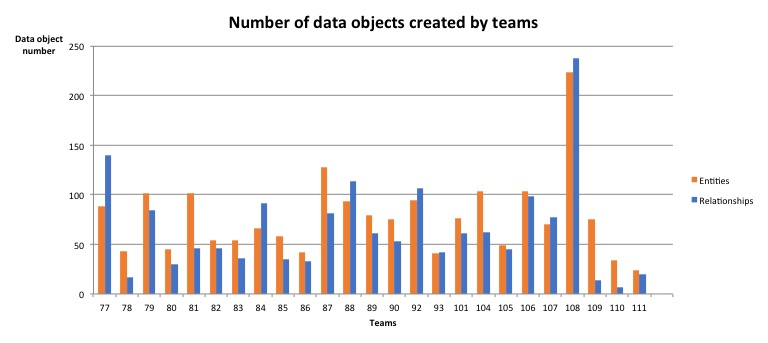
\includegraphics[height=1.5in]{img/user_created_objects}
	\caption{The number of entities and relationships that the groups created.}
	\label{fig:user_created_objects}
\end{figure}

The 25 teams created 1919 entities and 1636 relationships in total (Figure~\ref{fig:user_created_objects}). The number of entities each team created ranges from 24 to 223 (M=76, SD=40.2), and the relationships ranged from 7 to 237 (M=65, SD=49.1). One reason causing the wide variety is the usage of CAnalytics in the task (e.g. Team 111 did not use much of CAnalytics as other teams did), but the major reason is the different strategies teams took in approaching the task. Teams adopted different levels of granularity when collecting evidence. Figure~\ref{fig:network_example} shows two exemplar node-link graphs that illustrate the evidence two teams collected. Team 108 modeled suspect's every single action as an event, in an attempt to discover connections between robbery cases by examining similarities and dissimilarities in suspects' behavior patterns. In contrast, Team 107 only extracted high-level entities and modeled a whole robbery case as an event, resulting in many fewer data objects. The graph provides an overview of the seven cases and relationships among suspects. Neither strategy is better than the other, because they offer different insights and could be utilized in different stages of analysis. Two questions must be addressed here: 1. how should team members coordinate themselves to keep consistent with information granularity when collecting evidence; 2. how can the system provide a proper view for multiple levels of evidence granularity? The graph by Team 108 is obviously too noisy to provide insight. 

\begin{figure}
\centering
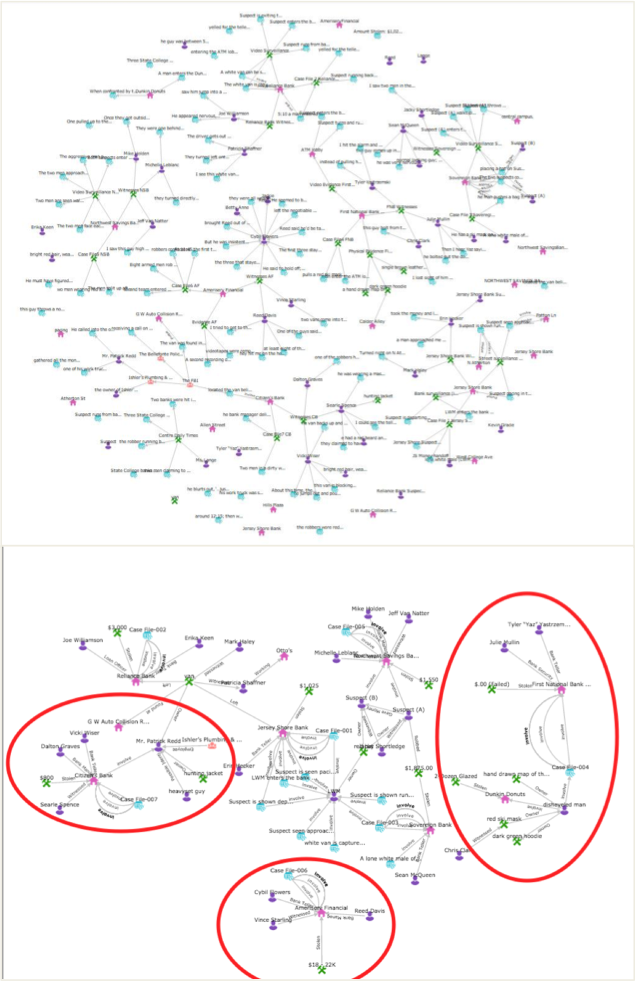
\includegraphics[width=0.7\linewidth]{img/network_example}
\caption{Two node-link graphs created by student analysts. The top one (by Team 108) contains a large number of nodes and links, describing every single action of suspected robbers. The bottom one (by Team 107) contains fewer nodes and links, describing only high-level events}
\label{fig:network_example}
\end{figure}

\hl{categorize entities inconsistently}
Another primary collaborative breakdown during evidence collection is inconsistency of data modeling. For example, some named entities could be modeled as different categories of data objects (e.g. a bank can be treated as an organization or a location). While such inconsistencies are superficial, they could lead to team confusion and misinterpretations. Such information serves as foundation for evidence schematization from which a team draws conclusion. 




\subsection{Collaborative Evidence Schematization}

Participants believed the visualization tools provided by CAnalytics facilitated the schematization and synthesis process. When they created a data object, the data was automatically laid out in multiple views. This changes their workflow from linear (first extract data and then visualize data) to parallel (create and view data objects). When a team is collecting evidence from the document, they are also organizing the document with sorted evidence. 

\begin{quote}
	\textit{`CAnalytics is helpful to our work because of its ability to edit the physical document with such organization. This with the combination of immediately adding all of the entities into a connected web that doesn't have to be manually created saves a lot of time'.} (P10)
\end{quote}

Another benefit students mentioned was that they no longer needed to create separate data structures redundantly for different analytic tools. To visualize different data types (e.g. spatial data, event data, linked data), analysts have multiple tools in their toolkit, yet different tools usually require different data formats. 

\hl{quote supporting the argument that team do not need to create separate models}

Besides, traditional visualization tools are usually designed for single user only. Thus teams had to divide work by tools; for example, one member creates an ACH matrix, and another member creates a node-link graph. The tool limit leads to loose coupled collaborative work; individuals work on their own and put together work in the end. 

\begin{quote}
	\textit{`we split the work by category: one would do the timeline, one would write up assumptions, and one would work on the IEW chart. We did this since all of us could not edit a single document at the same time.'}
\end{quote}

Using multiple tools also results in multiple scattered documents, making it difficult for teams to manage and organize.  

\begin{quote}
	\textit{`When we didn't have CAnalytics, we had a lot of different word documents that we had to share with each other in Google Doc. With CAnalytics, we were able to keep all the information, network, timeline, and BLUF analysis in one spot that we were all able to view at the same time as a group'.} (P58)
\end{quote}
\begin{quote}
	\textit{`CAnalytics made it easier to see everything mapped out in one place as opposed to doing it the old fashion way. It was way more convenient and efficient to have everything in one application'.} (P71)
\end{quote}


% The ease of sharing and putting work together also helps information analysis. Students found it helpful ``because I could see how all of our different ideas merged together to create our final product.'' Another student shared his experience about how the tool helped develop their theory. 


The positive feedback from the questionnaire is confirmed with system logs. We find that the usage of visualization tools is significantly correlated with team performance (r = .49, p < .05). Note we exclude Team 78, 79, 93, 109, and 111 as outliers as they did not use much of the tool. 

\begin{figure}
	\centering
	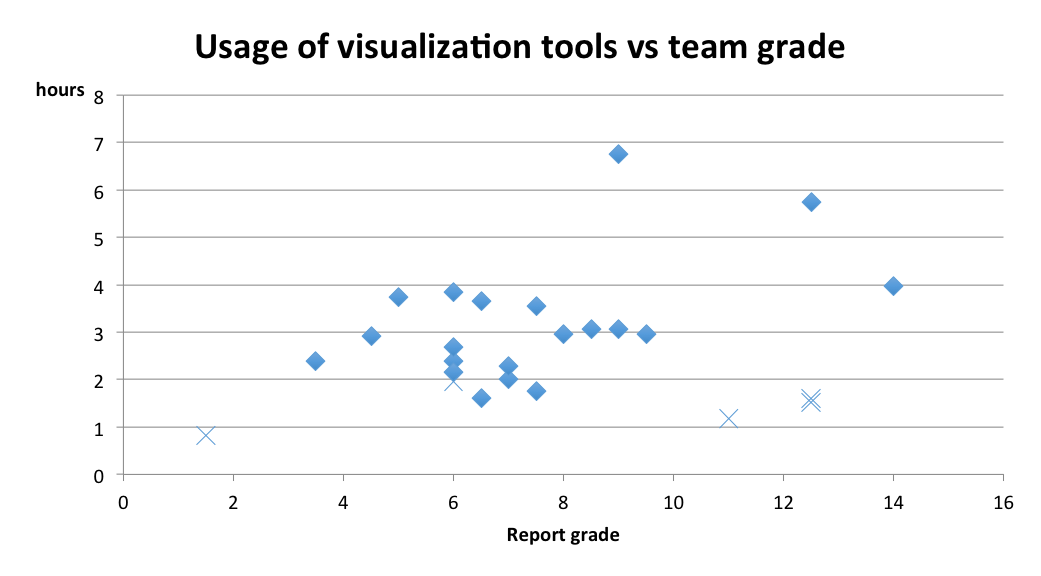
\includegraphics[height=1.5in]{img/vis_correlate_perf}
	\caption{Chart showing that team performance is highly correlated with usage of visualization tools (r = .49, p < .05). Crossings are outlier teams that do not use much of visualization tools}
\end{figure}

\hl{visualization usage??}
We then look into more specifically how teams used the visualization tools. Teams spent most time on the node-link graph. 

\begin{figure}
	\centering
	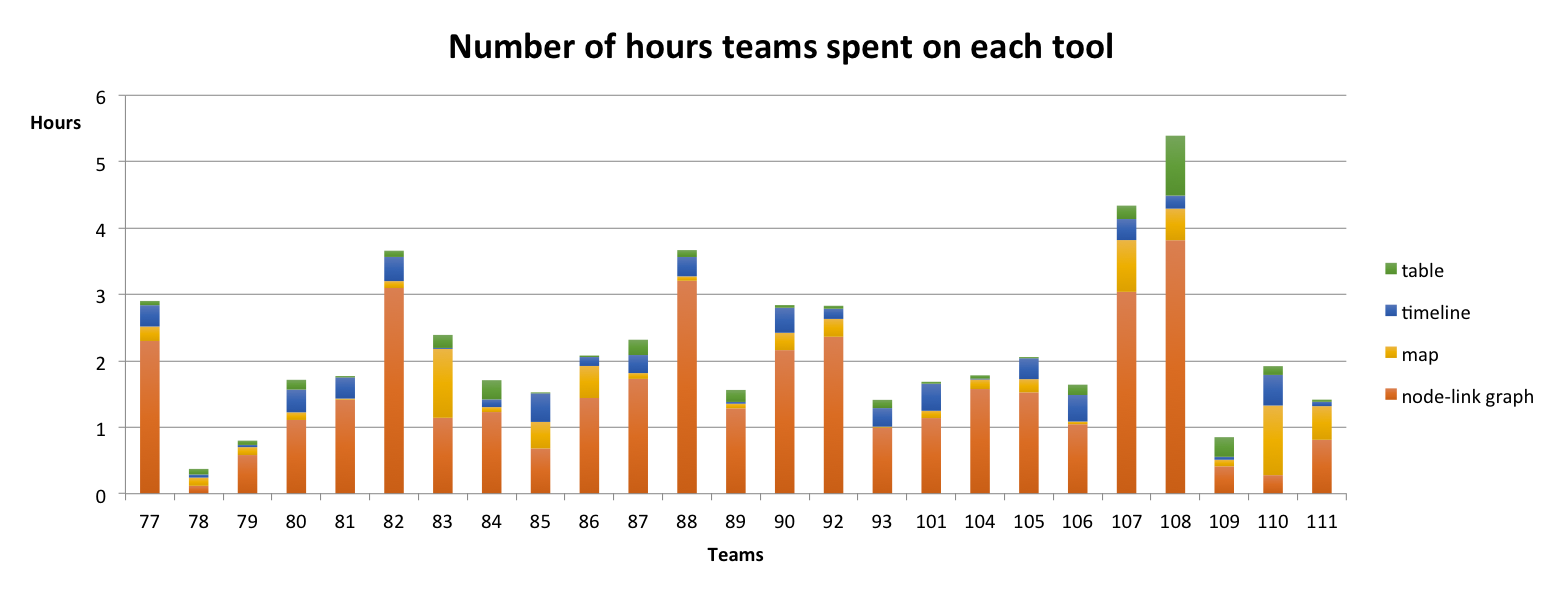
\includegraphics[height=1.5in]{img/vis_usage}
	\caption{Chart showing the usage of the visualization tools}
\end{figure}

When we look into the visualization products team created, we find several problems. For example, when information volume increases, it becomes challenging to distinguish useful information from background noise. As shown in the top graph in Figure~\ref{fig:network_example}, the node-link graph contains so many nodes that pattern discovery becomes very difficult.



%% reliability of information 
Another issue is difficulty to distinguish reliability of information. For example, while all displayed as valid connections in the node-link graph, some connections were literally specified in the original document, whereas others might be inferred. Analysts must be cautious about the different reliability of these connections when taking them for analysis. To avoid the issue, some groups only added most reliable facts to the shared view. While this approach kept the graph clean and free of noise, the team lost the chance to get inspired by and build upon each other's thought, which is of critical value in collaborative information analysis. Worse, the fear that adding a piece of less reliable information would mislead group thinking would discourage teammates to contribute. Mechanism to share and distinguish information of mixed reliability is needed.


Participants also complaint that not being able to share the schematization result makes their collaboration difficult. The current design allows individuals to arrange their own layout of evidence without interfering other member's sensemaking. However, while acknowledging the advantage of parallel sensemaking, participants requested to be able to share their visual product so that they can discuss based on the same ground.

\begin{quote}
	This was very hard to coordinate with my group members because we could be looking at the same information but arranged in completely different ways. (User 31)
\end{quote}




\subsection{Overall Coordination}

Teams had a mixture of collaborative settings. During class teams worked collocated and synchronously. When outside class, 15 teams (60\%) worked remotely, 5 teams collocated, and the other 5 teams had a mix of collocated and distributed work. In terms of time, only one team chose to work asynchronously. When asked how they coordinated work in class and outside class respectively, teams answered they accomplished different things: when in class, they worked closely on things that have high dependency, such as discussing overall direction, negotiating role division, and dividing work into loosely coupled modules. These work prepared them to be able to work on individual modules separately outside class. Teams reflected that it is easier to articulate opinions and analysis with face-to-face interactions as they require high-frequency conversation turns. Especially when team members have conflicted opinions, teams prefer to talk directly to reach an agreement. 

\begin{quote}
	Most of the work done outside of class was planned for and outlined when we could easily talk in class. Then we would continue what we had established while working apart from each other (P78)
\end{quote}

\begin{quote}
	We finished all of our annotations in class and had a good foundation of what we as a group believed went down…Once we had everything annotated through CAnalytics we primarily then worked via this tool and google docs to craft the final submission and bring everything together. We had a plan to meet up outside of class but found with a combination of these two tools we didn’t actually need to. (P148)
\end{quote}

\begin{quote}
	If we did not have CAnalytics, we probably would have had to meet in person. Even if we used Google docs, it would have been hard to coordinate all the work (P126)
\end{quote}


In the survey 88\% participants rated positively on team awareness, indicating that most of them felt aware of what their team members did. We then find that team self-reported awareness was significantly correlated with perceived performance, meaning that when individuals kept updated with other team member's activities, they felt more confident with their team performance. However, no correlation was found between awareness and team's real performance. 

The awareness features were received well. When asked what features helped them stay aware of team activities, 28 participants mentioned the tool coordinator, 24 mentioned the notification system, 19 mentioned the history tool, 14 mentioned the real-time update of user-generated data.  

\begin{quote}
The updates in the corner of the screen and the dot that appeared on the tabs was the primary way that helped me determine what my teammate was working on. For example, when there was a dot in the document tab, I knew that my teammate was working on annotating evidence. Also, if they were in the network tab, I knew that they were drawing inferences from the evidence we had collected. (User 166)
\end{quote}

\begin{quote}
	In CAnalytics there is a history tab where you can check all of the changes that were made and when so that my teammates and I could check the progress of the project and see who exactly was making changes to what.(U151)
\end{quote}

Besides, participants commented that being aware made them more engaged in the work. Being able to see teammate's real-time contribution motivates individuals to make equal or more contributions. 

\begin{quote}
the notifications every time you saw someone annotated something kept you peace at mind that your teammates are also working efficiently on this project. (U64)
\end{quote}
\begin{quote}
During class I wasn’t sure if my teammates were doing work for that class or another thing but then seeing their dot switch between applications on the software and updates pop up on my screen I knew they were doing work for 231. (U141)
\end{quote}
\begin{quote}
CAnalytics allowed us to see how much each person had contributed to their work (142)
\end{quote}






% discussion v2
\section{Discussion}

\subsection{Difference from prior work}

Our overarching research objective is to investigate software designs that better support the need of collaborative information analysis. The fluid settings of many team activities (synchronous/asynchronous, collocated/distributed), the complexity of their tasks, the need to analyze high-volume and complicated-structured data, make the task challenging. Current analytic teams have little support; most tools (e.g. PARC ACH and IBM Analyst's Notebook) are designed for single user and only part of the analysis process. By providing effective technology to aspects of information analysis (e.g. evidence collection, evidence schematization, hypothesis generation, and overall coordination), we can make analytic teams have more efficient workflow, better team performance, and more engaging work. 

In a comprehensive review of CSCW papers by \cite{Wainer2007}, they found that empirical papers can be evaluative, which describe an innovative groupware followed by a small part of evaluation, or descriptive, which describe team behavior in a work environment with or without an existing tool, but none combines development of an innovative groupware with detailed observation of team behavior applying the tool. This is possibly due to the great challenge in groupware assessment. As Stahl \cite{Stahl2006} put it, \textit{``To see how it really supports groups, groups must use it under relatively naturalistic conditions and for a long enough time to become comfortable with it. But this requires building a sufficiently complete and robust prototype for group usage, finding an appropriate group of users, training users in its use, and involving them in a meaningful application of the software that properly exercises the functionality of interest.''} (P. 197). Our study aims to fill in that void: a design research that implements an tool, observe how teams use it in a complex task, probe design implications, and iteratively improve the tool.

The goal is two-folds: 1. to design and evaluate the tool for supporting collaborative information analysis; 2. to use the tool as a means to probe how teams collaborate with technology mediation in complex tasks. The two goals serve each other: the result of the observation informs the design the of tool, and new implementation probes various aspects of team collaboration behavior for new insights.

Our study is close to real world scenarios in three aspects. First, our participants are students who are being trained to become professional analysts. User-centered design is essential to understand the challenges of information analysts \cite{Scholtz2014}. However, professional analysts are often limited to access due to security and confidential issues. Attempt to involve them in long-term design process as in our study is almost impossible. Instead, many researches recruit college students in their empirical study. However, these participants lack the advanced knowledge and skills (e.g. ACH, link analysis) that are often used. Our participants are mostly trained for three years in the program. Before the study, the students have taken nine weeks of the course, and have used PARC ACH, IBM Notebook, Evidence Matrix, and other analytic techniques to solve similar projects. They are familiar with the practice of the community.

Second, the task content is close to real world cases. The task is complex, containing seven cases, and involves various information sources (news media, social media, witness report, sensor data, etc.). Information can be of various reliability and credibility, requiring the analysts to investigate and judge. The task result is open-ended, similar to the real case which usually has no single answer. Analysts have to make their best hypotheses based on their provided information.

Third, the study context is similar to real world environment. Students have multiple courses and projects, similar to analysts who often are occupied in multiple work threads. Our participants have fluid collaborative settings (synchronous/asynchronous, collocated/distributed). This is similar to professional analysts, who often find themselves in different collaboration situations, depending on the physical constraint and their task needs.


\subsection{Implications for theory and design} 

\paragraph{Data collection as part of analysis}
A common misconception of information analysis is analysis of a specific set of data. Existing analytic techniques and tools such as ACH often assume that data has been modeled and can be applied directly to hypothesis development, but provide no support for data modeling at all. Analysts are treated as ``consumers'' of data.

However, we find that in our study participants spent a significant amount of time in determining collaboratively what to collect, what criteria to use, and what schema to model the annotations. These issues depend on what questions the team is to answer and how to answer the question. The team must collaboratively frame the question and decide the data gap to answer the question. Teams that failed to do ended up with inconsistent data models, which added difficulty to next-step analysis. 

Also, our log analysis reveals that data collection and data analysis are closely coupled along the process. Analysts do not work linearly from data collection to analysis, but work on both simultaneously and iteratively. As team's framing of their question evolves along time, their revise their evidence to support the frame. While prior works have observed the integrated process of data collection and analysis by qualitatively coding participant's behavior, our log analysis complements the finding by capturing and visualizing analysts' real interactions. 

% Views as team resources
\paragraph{Views as resources}

\hl{views should be sharable, reusable, extensible, collapsible, and comparable}

In addition to sharing of data, we find that views of data should become shareable resources as well. With the identical data pool, analysts often have different views of data. For example, analysts can apply a filter to have a reduced data view, highlight an area to sharpen analytic focus, and re-layout the node-link graph to cluster relevant entities. While the data pool represents the information the team have available, individual views of the data reflect analyst's \emph{interpretation} toward the information. Therefore we propose that just like data, views, which embodies interpretation of data, should be shareable. 

Views as resources should also be extensible, and reusable. For example, several participants reflected that there were situations when they found a collaborator's view useful and wanted to build their own work upon that view without manually reproducing the view. With views as resources, individuals can take the views to their need. They can also deliberatively share their own view when they feel other collaborators will be interested. Shared views are interactive rather than static images, so that analysts can still perform full functions including filtering and highlighting, and are able to evolve the view with collective team efforts, a critical requirement emphasized in \cite{Carroll2013}


We found that views should be treated as shareable resources. Complex cognitive and collaborative activities are often achieved through meaningful views of data, as externalization of human thought, offload of cognitive demand, and mediation of team cognition. In our current system, teams share the same data pool but have individual views of data. This was originally designed on purpose to enable individuals to have their own arrangement of data and to avoid interference. But we found flaw in such design as different views could hinder teams from collaboratively developing a theory. We propose that views should be another \emph{resource} in addition to others like data and tools, which could be shared, reused, and evolved. Teammates could deliberatively share their own view when they believe In our planned next version of tools, individuals still have personal views but can always share views as public resources. Teammates can take shared views for their own use and continue developing the views without duplicating it. This is different from public/private workspace as implemented in \cite{Convertino2011}, in which teams only have a single public space. With complex tasks multiple threads may be undertaken at the same time and sharing in one space may cause confusion. This is also different from what \cite{Nobarany2012} implemented as a means to facilitate reuse of views because their views are static images and limit the possibility to evolve with collective team efforts.


% collapse information
Several teams reflected that the node-link graph becomes difficult to read after the size of entities becomes large. Nodes and links are clustered in the view and get significant overlap. While applying a filter can always reduce the data, there are situations when analyst need to get an overview of the complete story without data filtered out. One way is to enable collapse of information. Connected nodes are often representing a same topic. An event node linked with a location, an organization, and several people nodes makes up a complete event. When details are not desired, these nodes can collapse into a single event node, or \emph{an evidence cluster}. The cluster can continued to be collapsed until there only exist several disconnected evidence clusters. The capability of collapsing and expanding information is important as it saves screen space and helps participants sharpen their analytic focus.

% views for side-by-side comparison
Several teams spontaneously created an evidence matrix (Figure~\ref{fig:evidence_matrix}) on a separate document. The matrix lists importance evidence for each crime case, and aligns them side by side. Such capability is missing in the tool as it provides a schema to compare cases and presents clear picture of the similarities and dissimilarities between cases. 

add with communication, mixed reliability 
We also found that certain mechanism of communication should be enabled when constructing shared views. In the current system, teammates contributed information of various reliability in the same view, causing confusion between facts and inferences. 

% view of uncertainty

\paragraph{Conflict as collaboration opportunity }

% Role of technology
\paragraph{Role of technology}
We reflect on the role of technology in mediating collaboration. 

Adoption of any technology will eventually change the workflow in teams. Teamwork is inevitably reorganized by the constraints of technology.

For example, by enabling the sharing of the same data models, CAnalytics ``forces'' teams to work in a closer-coupled way. With traditional tools, teammates have separate tools and model separate data structures for each tool. The way one individual formats data does not directly affect his teammate's schematization. In CAnalytics, however, if team members employ different rules of collecting evidence, the team will end up with inconsistent data models, which eventually impedes analysis. To accommodate to such tool constraint, the team must work more closely, ensuring an agreement of strategy of evidence collection.

Both the users and designers of collaborative tools must be cautious not to be too ambitious of tools. Tool users must realize that the tool only ``mediates'' team collaboration, but does not ensure smooth collaboration. For example, two teams in our study reflected that their team conversation decreased dramatically compared to previous project because they felt they knew teammates' activities through the tool and ``there seems no need to talk'' (P??), but the lack of communication eventually harmed their collaboration. Designers, on the other hand, should be aware that technology is not support every aspect of collaborative information analysis. From our study, we find three aspects that technology could play a significant role apart from data sharing:

1. provide feedback. Team work consists of two major phases: establishing a plan and executing a plan. When the teams are establishing a plan, they discuss team's overall goal, strategies and tactics to reach the goal, resources available, and role responsibilities. This process usually requires high frequency of conversation turns, and is more effective in face-to-face communication. Participants in our study spent a significant amount of time in class on discussing the plan. During the execution of the plan, individuals perform their responsible parts of the plan. A critical part is to provide evidence from which individual's level of understanding of the plan can be inferred. Such evidence is usually given off as a side effect of action without extra verbal effort in face-to-face settings: a correct action indicates understanding whereas a wrong action or failure to act indicates misunderstanding. In remote settings, however, deliberative signaling needs to be designed. Technology can help in relaying such information when the user interacts with the system. For example, the tool coordinator in our tool provides visual feedback on where teammates are working and the notification system streams live changes teammates made. These updates help teammates monitor whether collaborators have understood the team plan. The feedback is effective because users do not need to explicitly state their understanding of the plan. 


2. makes teamwork engaging. A positive emerging finding is that the collaborative tool seemed to increase Participant's engagement. Students stated that seeing teammates' real-time activities and their own activities being exposed to teammates motivated them to contribute, made them peace at mind, and increased their accountability. This finding is worth attention as group work is often blamed for \emph{social loafing} \cite{Karau1993},  referring to the problem that individuals tend to work less hard when in a group than when they are working as individuals. Our finding provides evidence that appropriate awareness design is likely to reduce that effect, and may even make teamwork engaging. The finding could have direct impact on education---not only the education of information analysis as in our study, but also education of other domains as well: technology that enables collaborative learning could increase students' engagement (e.g. \cite{zheng2015}). 


3. turn conflict into cooperative activities. While our participants believe they are more willing to communicate directly over conflicts, technology can assist in detecting such conflicts and turn them into opportunities for cooperative activities. 

\paragraph{Managing affordances in opportunist coupling}

\paragraph{Narrowing down data}

\paragraph{Deletion as contribution}

% Deletion from artifact is socially difficult, compare to wiki but should relate to CIA task. 
% Make deletion socially acceptable
We found that compared to ``adding'' data to the tool, participants had more difficulty in ``deleting'' things, especially when they were created by other people. Such difficulty was not technically, but socially. For example, we found from the system log that when an individual updates a relationship between two entities that is either incomplete or conflicting, s/he usually creates a new relationship with the updated information without modification or deletion of the old one. We imagine that the reason behind is that deleting other's work is showing disagreement to teammates, which could cause discomfort to both sides \cite{Asch1951}. The problem occurs in other domains as well, for example, in Wiki collaboration \cite{grudin2010}, where people feel uncomfortable deleting other member's writing. Usually a version control system is employed so that prior contribution is always available even after deleted. However,the issue was more complex in the context of information analysis as the task itself and data types involved in the task are more complex than text. A possible way to reduce the effect is to weaken the indicator of disagreement. For example, instead of permanently deletion, users can ``archive'' an object for later use, or temporarily hide objects. 

% We also observed that compared to ``adding'' things to shared artifact, participants had more difficulty ``deleting'' things. Such difficulty was not technically, but socially. For example, we found in the system log that instead of deleting an old link created by a teammate, the user created another link with updated information. We imagine that by deleting other's work, people feel they are denying teammate's contribution. Such disagreement can easily make both sides uncomfortable \cite{Asch1951}. Keeping out-of-date information, however, unnecessarily complicated the shared artifact, and confused them eventually with mixed information. 




\section{Conclusion}
\hl{not modified yet}

% Limitation
In this paper, we present findings from a classroom study in which teams of information analysts in training collaboratively completed a complex intelligence project mediated by our tool. As collaborative information analysis is increasingly a typical and chronic task, it is important for research to examine, understand, and provide effective tools and environments for these long-term, real-world CSCW interactions. This requires situating research in more complex work activity contexts, and directly investigating interactions, experiences, and outcomes in those contexts. Our classroom study provides initial results on team interactions mediated by advanced technology over extended time periods. The encouraging results motivate us to continue refining and re-evaluating the tool.

Meanwhile, due to the nature of classroom study, a lot of variables that cannot be factored could influence the result. For example, students coordinated teamwork not only through CAnalytics but also through face-to-face meeting. What the teams did outside CAnalytics is not collected, which obviously influenced team performance. But our work provides a realistic picture of usage of a collaborative tool in real world, and poses several design questions and hypotheses, which could be investigated in future controlled lab studies. 

%Since the study was conducted in a naturalist environment, participants were not observed in a controlled lab, and they were free to choose either face-to-face collaboration settings or remote work settings, and they could also use any other tools they preferred. Thus their high rating of awareness in the survey is not a sufficient proof of the success of the tool. Still, their answer in the open-ended questionnaire explained to some extent how the tool helped achieve the function.  
%
%
%establish the dots and connect the dots
%
%
%
%This paper talks about strength and weakness of lab and field study, and suggests combining the two methods. 
%A laboratory method for studying activity awareness. Convertino. 2004

\section{Acknowledgments}

To be added

% Balancing columns in a ref list is a bit of a pain because you
% either use a hack like flushend or balance, or manually insert
% a column break.  http://www.tex.ac.uk/cgi-bin/texfaq2html?label=balance
% multicols doesn't work because we're already in two-column mode,
% and flushend isn't awesome, so I choose balance.  See this
% for more info: http://cs.brown.edu/system/software/latex/doc/balance.pdf
%
% Note that in a perfect world balance wants to be in the first
% column of the last page.
%
% If balance doesn't work for you, you can remove that and
% hard-code a column break into the bbl file right before you
% submit:
%
% http://stackoverflow.com/questions/2149854/how-to-manually-equalize-columns-
% in-an-ieee-paper-if-using-bibtex
%
% Or, just remove \balance and give up on balancing the last page.
%
\balance{}


% REFERENCES FORMAT
% References must be the same font size as other body text.
\bibliographystyle{SIGCHI-Reference-Format}
\bibliography{sigproc}

\end{document}

%%% Local Variables:
%%% mode: latex
%%% TeX-master: t
%%% End:
